\section{Auswertung}
Kern der Auswertung ist die Bestimmung der Absorptionskoeffizienten und damit die Deutung der einzelnen Elementarwürfel aus Würfel 4.
Dafür wird in den ersten Schritten Aufschluss über die ersten drei Würfel durch Mittellung der eindeutigen Absorptionskoeffizienten erlangt. 
In passender Literatur \cite{wqs} finden sich Referenzwerte dieser Koeffizienten wodurch sich die hier verwendeten Materialien finden lassen.  
Folglich wird die Auswertung in vier Teile aufgebaut, die sich jeweils mit einem Würfel befasst. 

\subsection{Würfel 1-3}
Die Messreihen für den ersten Würfel dienen, da dieser nur aus einer Ummantelung besteht, der Bestimmung des Absorptionskoeffizienten für Alluminium und somit einer Bestimmung 
für die Intensität $I_0$. Da alle nachfolgenden Würfel ebenfalls aus dieser Ummantelung bestehen bleibt dieser $I_0$-Wert für alle Messungen gleich. Bei der Bestimmung des Absorptionskoeffizienten für die Alluminiumhülle
wird die Intensität ohne Würfel als $I_0$ verwendet. 
Die Strecke die der Strahl durch das Material bewältigen muss ist die doppelte Dicke der Ummantelung also
\begin{equation*}
    \increment x = \SI{2}{\milli\meter}.
\end{equation*}
Die Gleichung \eqref{eqn:hierlol} reduziert sich für die ersten drei Würfel auf einen Term. Dieser lässt sich schreiben als
\begin{equation*}
\mu = - \text{ln} \left( \frac{I(\increment x)}{I_0} \right) \frac{1}{\increment x}.
\end{equation*}
Mit den gemessenen Zählraten aus Tabelle \ref{tab:1} lassen sich nun die Absorptionskoeffizienten bestimmen. Diese ergeben sich zu
\begin{align*}
\mu_{\text{Würfel 1}} &= \SI{0.270(60)}{\per\centi\meter},\\
\mu_{\text{Würfel 2}} &= \SI{0.055(4)}{\per\centi\meter},\\
\mu_{\text{Würfel 3}} &= \SI{1.080(90)}{\per\centi\meter}. 
\end{align*}
\subsection{Würfel 4}
Für diesen Würfel wird die Matrix $A$ aus Gleichung \eqref{eqn:lul} verwendet. Außerdem kann bereits über Matrizenrechungen der Term $x = (A^{\text{T}}A)^{-1} A^{\text{T}}$ berechnet werden. Dieser ergibt sich zu

\begin{figure}
\centering
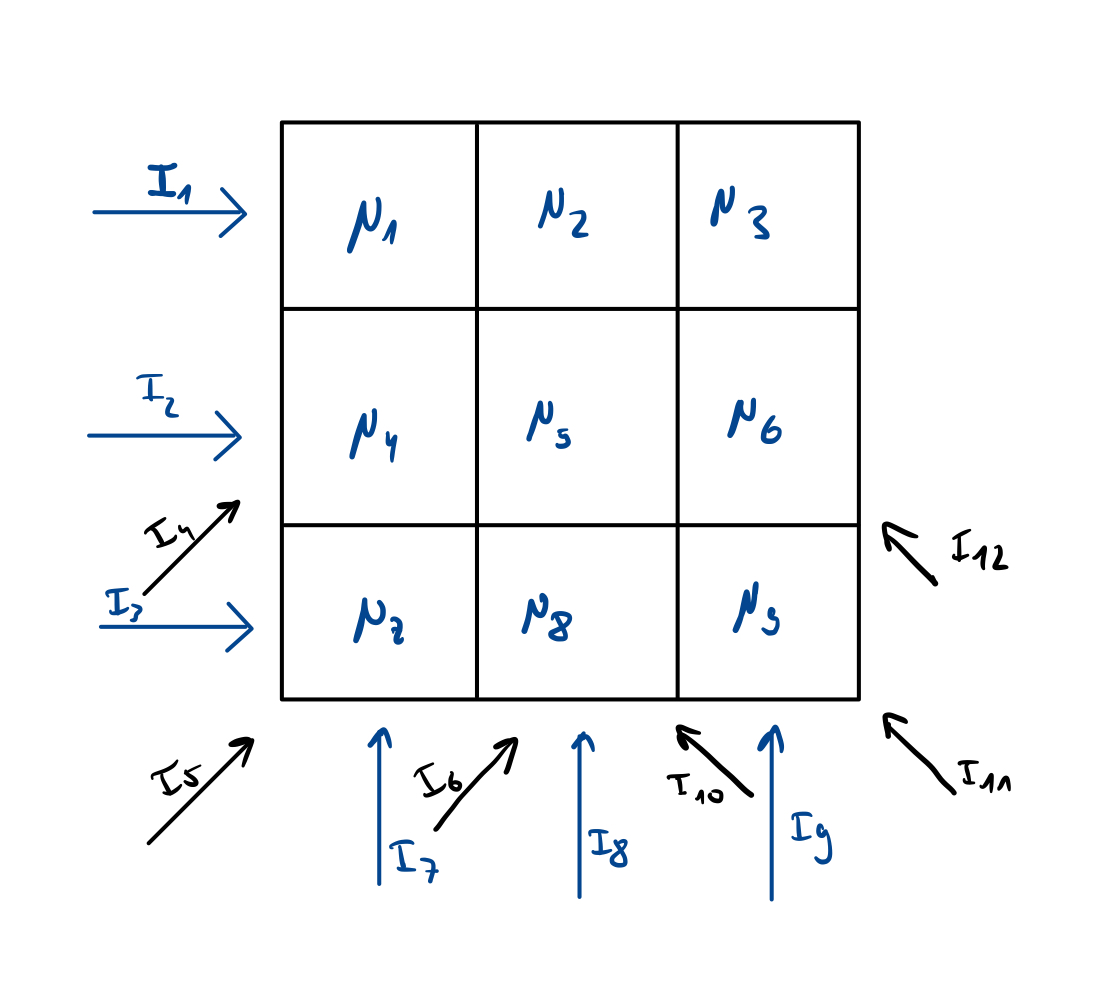
\includegraphics[width=0.6\textwidth]{bilder/file.jpg}
\caption{Schematische Anschauung zur Verdeutlichung der verschieden Projektionen und der entsprechenden Strahlausrichtung.}
\end{figure}

\setcounter{MaxMatrixCols}{20}
\begin{equation*}
    x =
\begin{pmatrix}
    \frac{14}{41} & \frac{-11}{164} & \frac{-13}{82} & \frac{-\sqrt{2}}{164} & \frac{13\sqrt{2}}{82} & \frac{-\sqrt{2}}{164} & \frac{-13}{82} & \frac{-11}{164} & \frac{14}{41} & \frac{39\sqrt{2}}{328} & \frac{-15\sqrt{2}}{164} & \frac{-43\sqrt{2}}{328} \\
    \frac{25}{246} & \frac{-16}{123} & \frac{25}{246} & \frac{57\sqrt{2}}{328} & \frac{-3\sqrt{2}}{164} & \frac{-25\sqrt{2}}{328} & \frac{-8}{123} & \frac{25}{123} & \frac{-8}{123} & \frac{-25\sqrt{2}}{328} & \frac{-3\sqrt{2}}{164} & \frac{57\sqrt{2}}{328} \\
    \frac{14}{41} & \frac{-11}{164} & \frac{-13}{82} & \frac{-43\sqrt{2}}{328} & \frac{-15\sqrt{2}}{164} & \frac{39\sqrt{2}}{328} & \frac{14}{41} & \frac{-11}{164} & \frac{-13}{82} & \frac{-\sqrt{2}}{164} & \frac{13\sqrt{2}}{82} & \frac{-\sqrt{2}}{164} \\
    \frac{-8}{123} & \frac{25}{123} & \frac{-8}{123} & \frac{-25\sqrt{2}}{328} & \frac{-3\sqrt{2}}{164} & \frac{57\sqrt{2}}{328} & \frac{25}{246} & \frac{-16}{123} & \frac{25}{246} & \frac{-25\sqrt{2}}{328} & \frac{-3\sqrt{2}}{164} & \frac{57\sqrt{2}}{328} \\
    \frac{-11}{82} & \frac{19}{82} & \frac{-11}{82} & \frac{-\sqrt{2}}{41} & \frac{11\sqrt{2}}{82} & \frac{-\sqrt{2}}{41} & \frac{-11}{82} & \frac{19}{82} & \frac{-11}{82} & \frac{-\sqrt{2}}{41} & \frac{11\sqrt{2}}{82} & \frac{-\sqrt{2}}{41} \\
    \frac{-8}{123} & \frac{25}{123} & \frac{-8}{123} & \frac{57\sqrt{2}}{328} & \frac{-3\sqrt{2}}{164} & \frac{-25\sqrt{2}}{328} & \frac{25}{246} & \frac{-16}{123} & \frac{25}{246} & \frac{57\sqrt{2}}{328} & \frac{-3\sqrt{2}}{164} & \frac{-25\sqrt{2}}{328} \\
    \frac{-13}{82} & \frac{-11}{164} & \frac{14}{41} & \frac{39\sqrt{2}}{328} & \frac{-15\sqrt{2}}{164} & \frac{-43\sqrt{2}}{328} & \frac{-13}{82} & \frac{-11}{164} & \frac{14}{41} & \frac{-\sqrt{2}}{164} & \frac{13\sqrt{2}}{82} & \frac{-\sqrt{2}}{164} \\
    \frac{25}{246} & \frac{-16}{123} & \frac{25}{246} & \frac{-25\sqrt{2}}{328} & \frac{-3\sqrt{2}}{164} & \frac{57\sqrt{2}}{328} & \frac{-8}{123} & \frac{25}{123} & \frac{-8}{123} & \frac{57\sqrt{2}}{328} & \frac{-3\sqrt{2}}{164} & \frac{-25\sqrt{2}}{328} \\
    \frac{-13}{82} & \frac{-11}{164} & \frac{14}{41} & \frac{-\sqrt{2}}{164} & \frac{13\sqrt{2}}{82} & \frac{-\sqrt{2}}{164} & \frac{14}{41} & \frac{-11}{164} & \frac{-13}{82} & \frac{-43\sqrt{2}}{328} & \frac{-15\sqrt{2}}{164} & \frac{39\sqrt{2}}{328} \\
\end{pmatrix}
\end{equation*}
Die Messungen der Intensitäten entlang der Projektionen des Würfels, die an der Matrix $A$ von oben nach unten schauend ersichtlich sind, stehen in der Tabelle \ref{tab:1}. 
Sie werden, wie nach der rechten Seite von Gleichung \eqref{eqn:hierlol} ersichtlich, mit dem Logarithmus und der Intensität $I_0$ modifiziert. Es ergibt sich somit der Vektor
\begin{equation*}
\vec{I} = 
\begin{pmatrix}
    \SI{1.296(31)}{} \\ 
    \SI{1.227(30)}{} \\ 
    \SI{1.321(31)}{} \\ 
    \SI{1.560(34)}{} \\ 
    \SI{1.771(38)}{} \\ 
    \SI{1.460(33)}{} \\ 
    \SI{0.220(20)}{} \\ 
    \SI{3.292(78)}{} \\ 
    \SI{0.228(20)}{} \\ 
    \SI{1.517(34)}{} \\ 
    \SI{1.762(38)}{} \\ 
    \SI{1.596(35)}{} \\ 
\end{pmatrix}.
\end{equation*}
Aus Matrixmultiplikation der beiden folgt nun 
\begin{equation*}
\vec{\mu} = 
\begin{pmatrix}
    \SI{0.075(30)}{\per\centi\meter} \\ 
    \SI{1.110(29)}{\per\centi\meter} \\ 
    \SI{0.064(35)}{\per\centi\meter} \\ 
    \SI{0.024(39)}{\per\centi\meter} \\ 
    \SI{1.095(28)}{\per\centi\meter} \\ 
    \SI{0.032(41)}{\per\centi\meter} \\ 
    \SI{0.116(42)}{\per\centi\meter} \\ 
    \SI{1.046(28)}{\per\centi\meter} \\ 
    \SI{0.118(42)}{\per\centi\meter} \\ 
\end{pmatrix}.
\end{equation*}
Die Zuordnungen der Absorptionskoeffizienten sind in der folgenden Tabelle \ref{tab:wurfel4} eingetragen.
\begin{table}
    \centering
    \caption{Absorptionskoeffizienten und Zuordnungen des zusammengesetzten Würfels.}
    \label{tab:wurfel4}
    \begin{tabular}{c c c c c}
      \toprule
      {Index} & $\mu$ [$\si{\per\centi\meter}$] & {Material}
                & Literatur & Abweichung [$\SI{}{\percent}$]\\
      \midrule
       1 & $\SI{0.075(30)}{}$ & Holz  & 0,052 & 40.0  \\
       2 & $\SI{1.110(29)}{}$ & Blei  & 1,174 & 5.5  \\
       3 & $\SI{0.064(35)}{}$ & Holz  & 0,052 & 20.0  \\
       4 & $\SI{0.024(39)}{}$ & Holz  & 0,052 & 50.0  \\
       5 & $\SI{1.095(28)}{}$ & Blei  & 1,174 & 6.7  \\
       6 & $\SI{0.032(41)}{}$ & Holz  & 0,052 & 40.0  \\
       7 & $\SI{0.116(42)}{}$ & Holz  & 0,052 &  120.0  \\
       8 & $\SI{1.046(28)}{}$ & Blei  & 1,174 & 10.9  \\
       9 & $\SI{0.118(42)}{}$ & Holz  & 0,052 & 130.0  \\
      \bottomrule
    \end{tabular}
\end{table}
